
\section{Communication Quality APIs}

We have exposed only a fundamental subset of the Communication Quality APIs on our gateway, similar to what we have done with our other sets of APIs. We chose this course of action for two reasons: one, due to the available tools IT provided us, and two, focusing on the most important capabilities for our primary use case.

Correspondingly, our implementation targets a subset of this API family: Quality on Demand, Quality on Demand Provisioning, and Quality of Service Profiles. These three services together provide dynamic quality adaptation, the provisioning of quality levels on an as-needed basis, and the specification of service profiles that ensure performance bounds for communications. By focusing our efforts there, we’ve created a lightweight, yet extremely efficient, collection of quality-management APIs that play well with our underlying infrastructure.

\subsection{Quality on Demand}

The Quality on Demand (QoD) API offers a programmable interface that allows developers to request stable latency or prioritized throughput managed directly by the network. By abstracting the complexity of underlying network technologies, the API enables developers to concentrate on optimizing user experiences for applications requiring high-performance network communication.

The solution employs 3GPP’s \emph{Nnef\_AFsessionWithQoS} interface to drive dynamic, on-demand subscription for application-level data flows. As an application client requires guaranteed QoS to a particular server, the client-side gateway collects the proper identifiers (i.e., client IP address, server IP address, port numbers) and translates them into standardized 3GPP flow description. This flow description is passed as a subscription request to the NEF (Network Exposure Function) through its \emph{Nnef\_AFsessionWithQoS} operation. The NEF checks the request against the existing network policy and available resources, and sends an authorization response stating whether the QoS resources were reserved successfully or not. If granted, the network dynamically applies the agreed QoS parameters end-to-end between the server and the application client.

In addition to session creation, the CAMARA QoD API provides functionality to manage active sessions. It allows retrieving session information by session ID or by device identifier, making it easier to monitor ongoing QoS allocations. Furthermore, the API supports extending the lifetime of existing sessions if continued QoS is required, as well as deleting sessions when QoS is no longer needed or the application session terminates.

\begin{figure}[H]
	\centerline{
		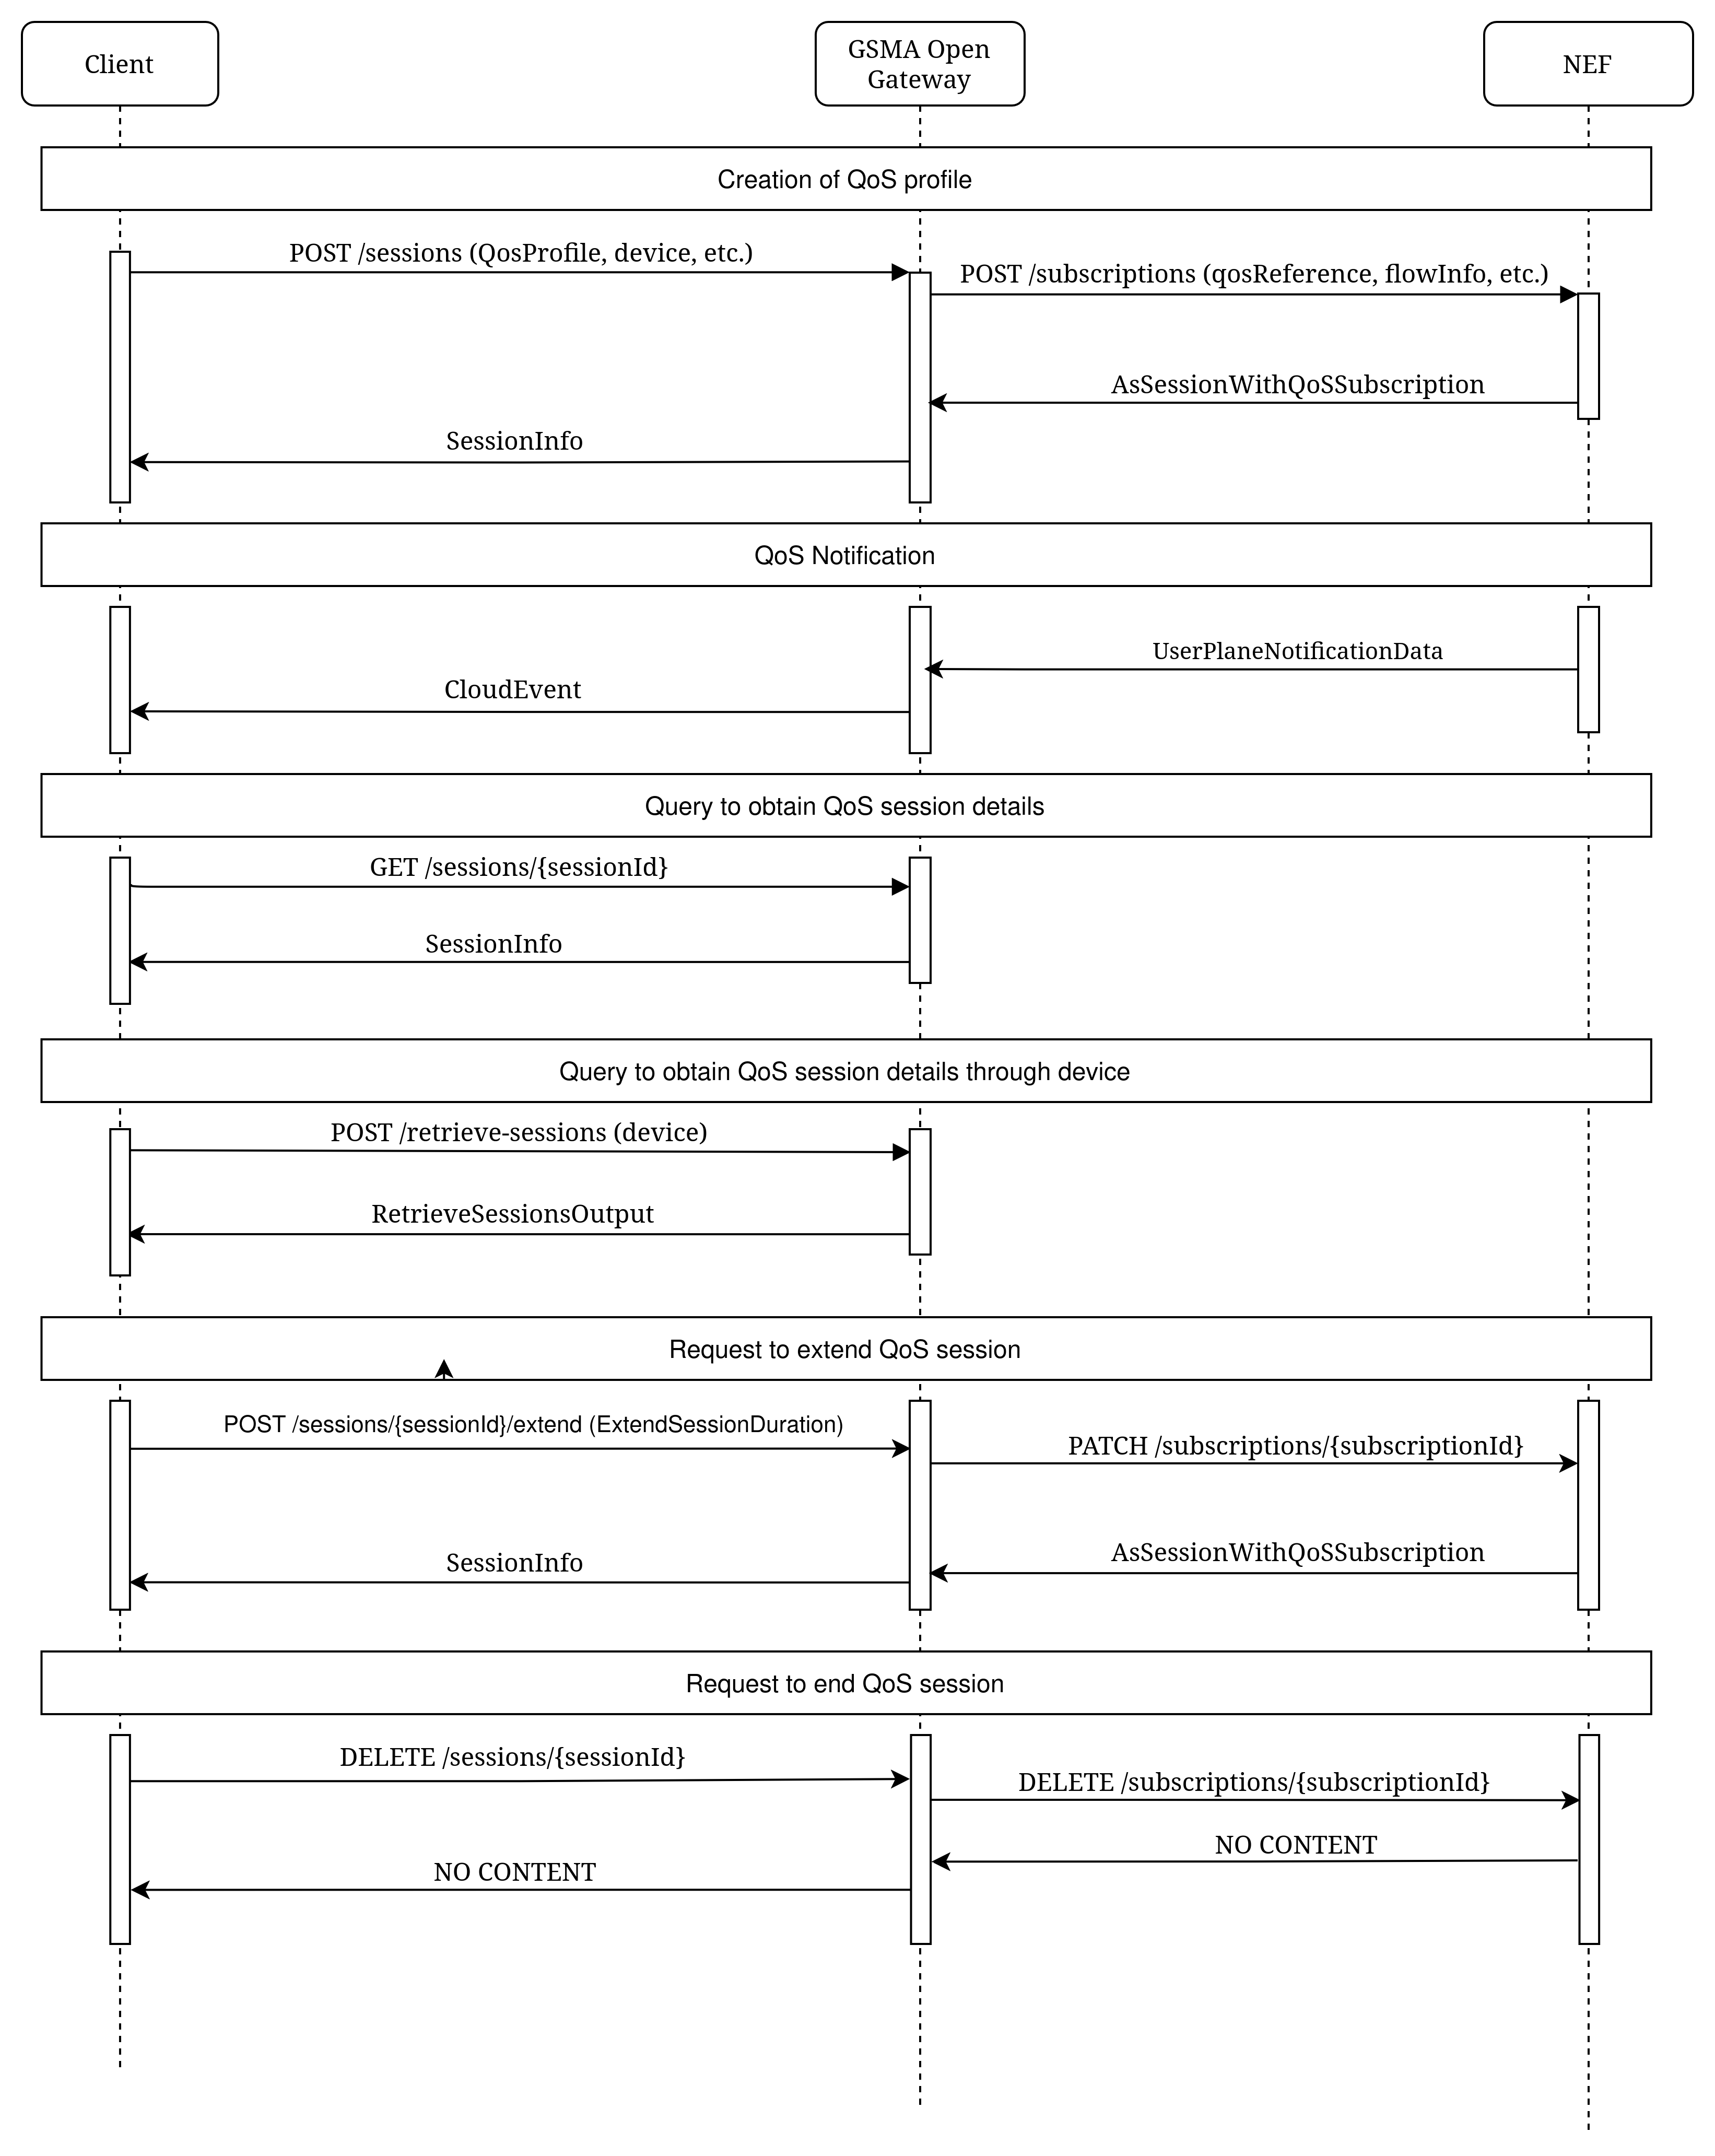
\includegraphics[width=10cm]{figs/QoD_sequence_diagram.png}
	}
	\caption{Quality on Demand Sequence Diagram}
\end{figure}

\subsection{Quality on Demand Provisioning}

The Quality On Demand Provisioning API provides a programmable interface that enables developers to assign specific Quality of Service (QoS) profiles to individual devices on a permanent basis. Once provisioned, the network applies the designated QoS profile to the device whenever it connects, maintaining the configuration until the provisioning is explicitly removed.

Similar to the previous Quality-on-Demand API, the QoD Provisioning API also leverages 3GPP’s \emph{Nnef\_AFsessionWithQoS} interface to manage QoS sessions. However, unlike the standard QoD API which typically focuses on application-level flows between clients and servers, the QoD Provisioning API is designed to allocate QoS resources directly for a specific device.

In this case, the gateway or application provides the device identity (e.g., SUPI, GPSI, or IP address) along with the requested QoS reference. The API translates this information into a 3GPP compliant request and submits it via the \emph{Nnef\_AFsessionWithQoS} interface to the NEF. The NEF evaluates network resource availability and policy constraints, and returns a response indicating whether the requested QoS resources have been successfully allocated for the device.

Similar to the QoD API, the QoD Provisioning API also provides management capabilities: it allows retrieving existing provisioning information by provisioning ID or device or deleting provisioning when the dedicated QoS is no longer required.


\begin{figure}[H]
	\centerline{
		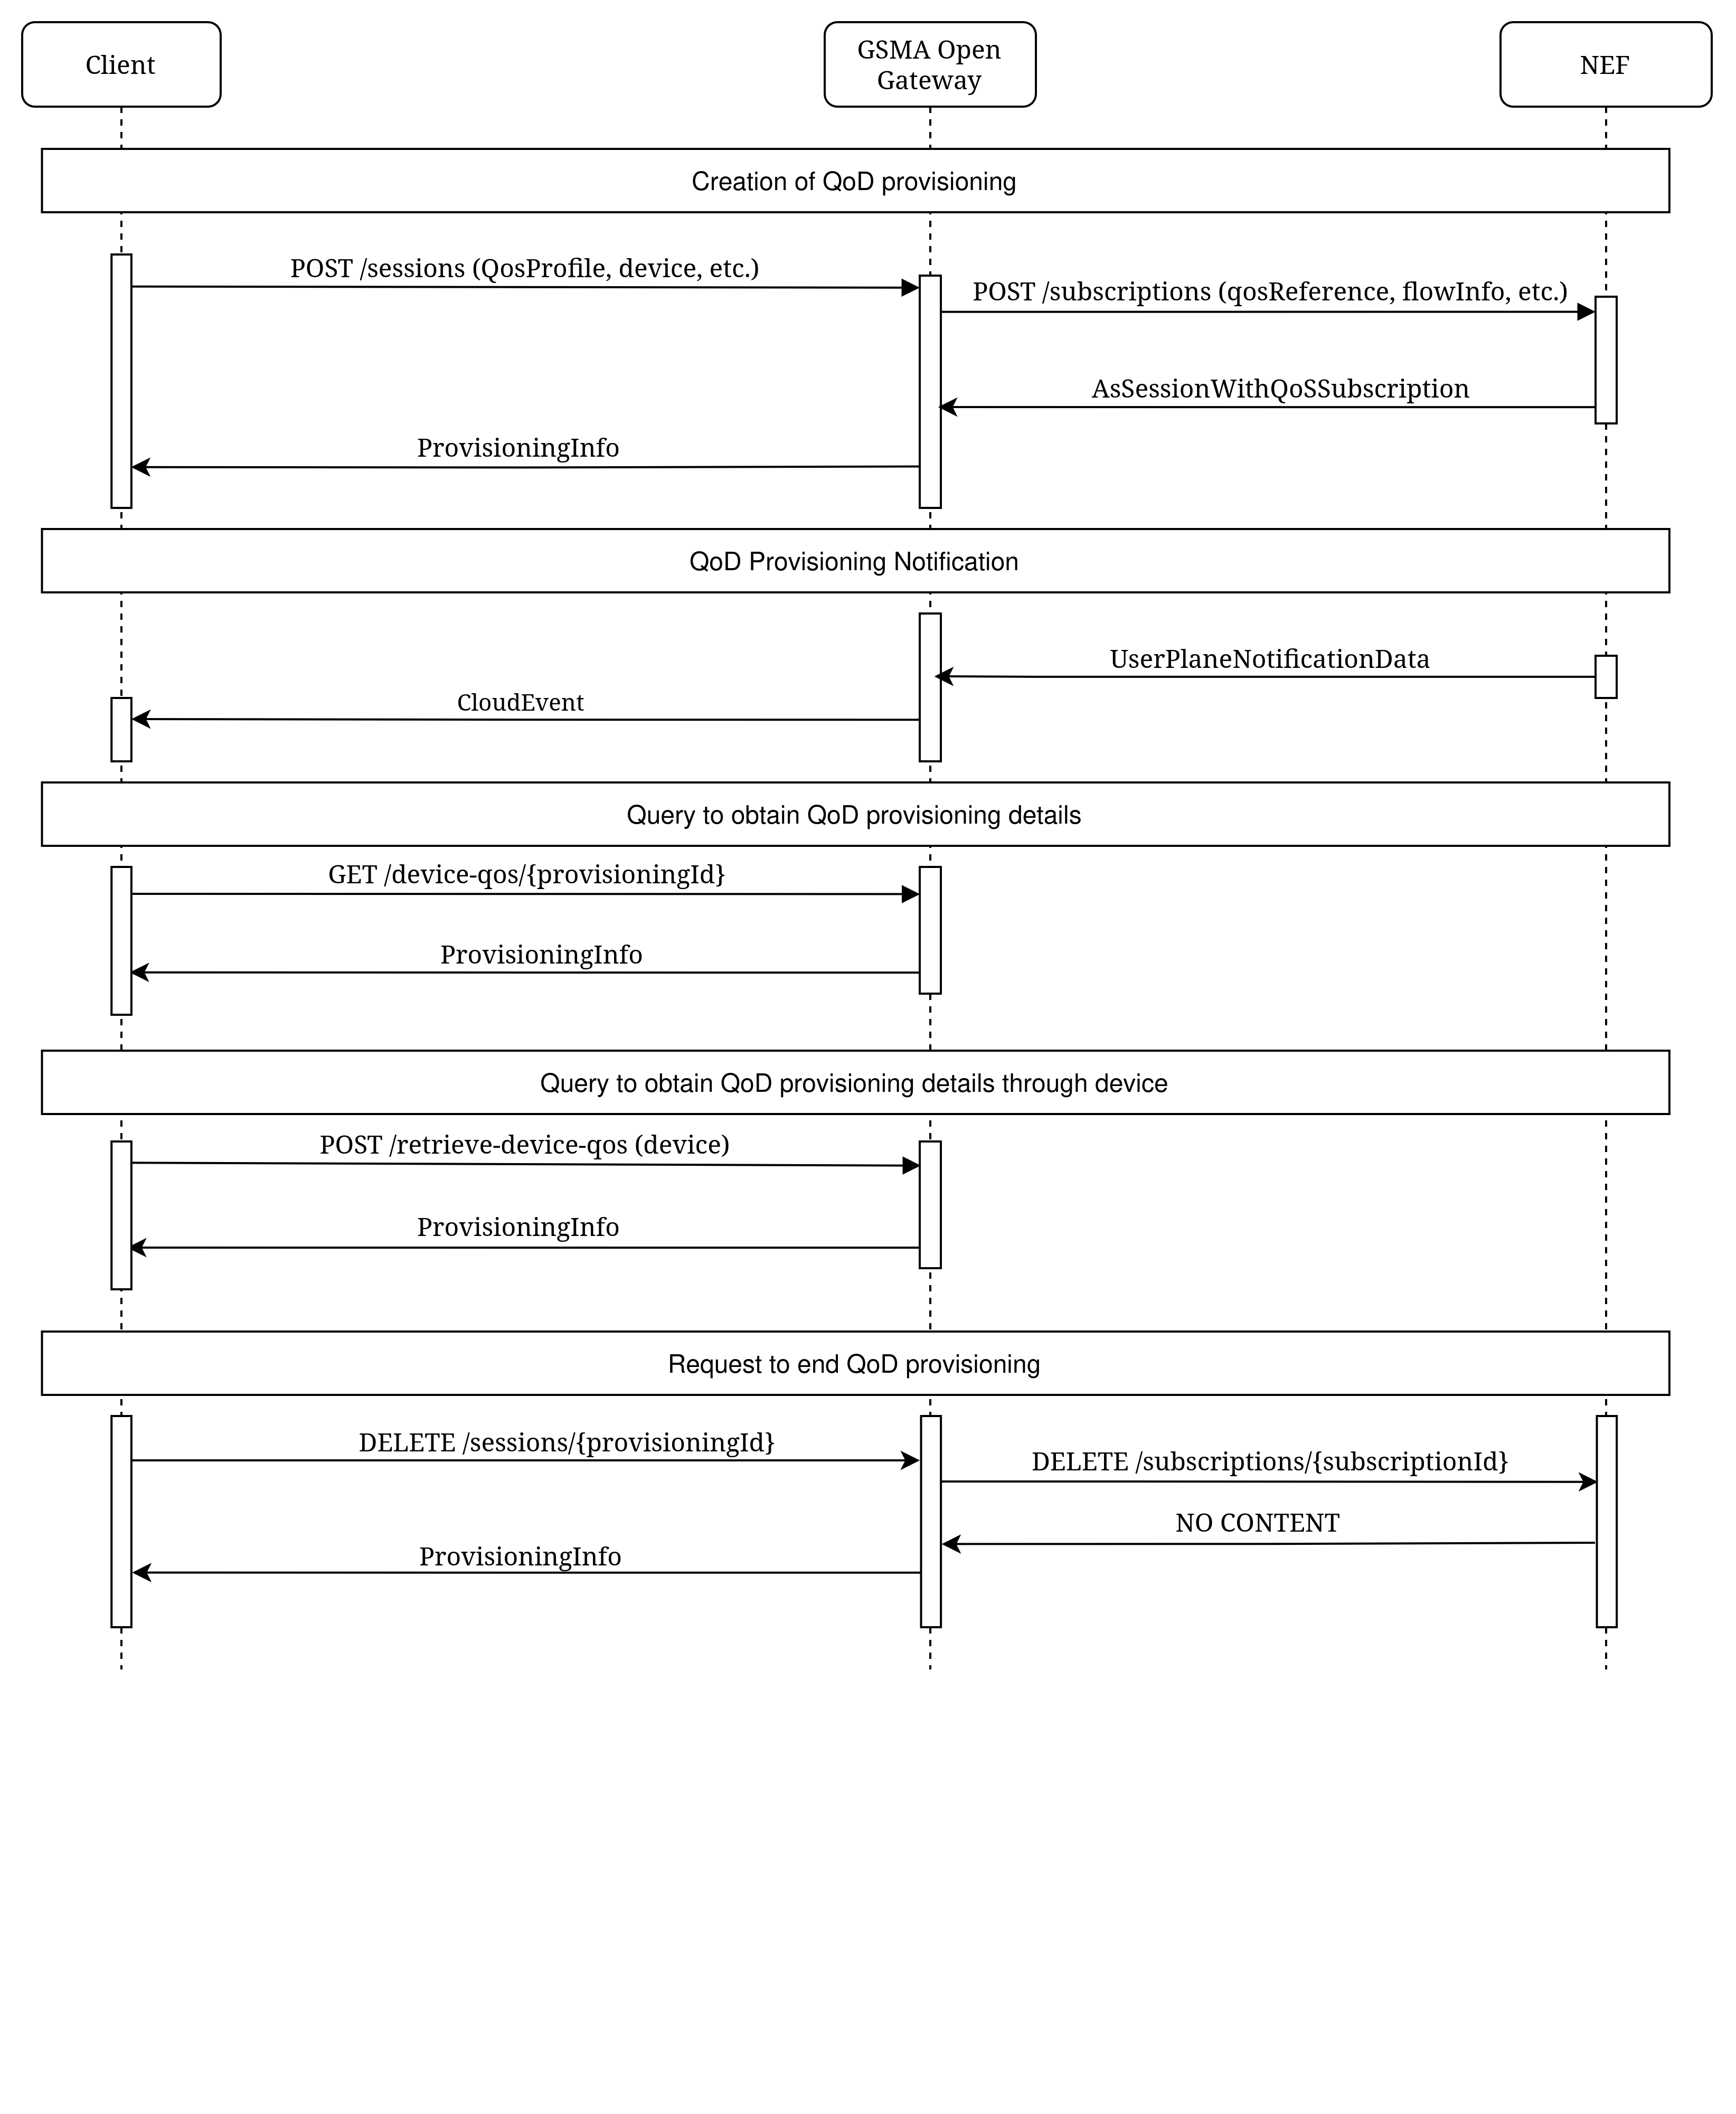
\includegraphics[width=10cm]{figs/QoD_prov_sequence_diagram.png}
	}
	\caption{Quality on Demand Provisioning Sequence Diagram}
\end{figure}

\subsection{Quality of Service Profiles}

The Quality-of-Service (QoS) Profiles API provides a collection of predefined network performance profiles, each identified by a unique name and characterized by parameters such as latency, throughput, and priority. These profiles enable application developers to define the desired network behavior for their application's data traffic, ensuring optimal and consistent performance. When used in conjunction with the Quality On Demand API, developers can request stable latency (reduced jitter) or prioritized throughput for specific data flows between client devices and application servers.

For this API, the NEF’s \emph{qosCharacteristics} interface is used to retrieve information about available QoS profiles. Depending on whether a specific QoS profile name is provided, the interface returns either the details of the requested profile or a list of all available QoS profiles and their information. The gateway processes the client’s request, making a request to the NEF interface. The NEF then responds with the corresponding QoS profile information, which the gateway then calculates the necessary parameters, and translates them into a compliant CAMARA's response, which can be used by the application to select appropriate QoS parameters for subsequent resource allocation requests.

\begin{figure}[H]
	\centerline{
		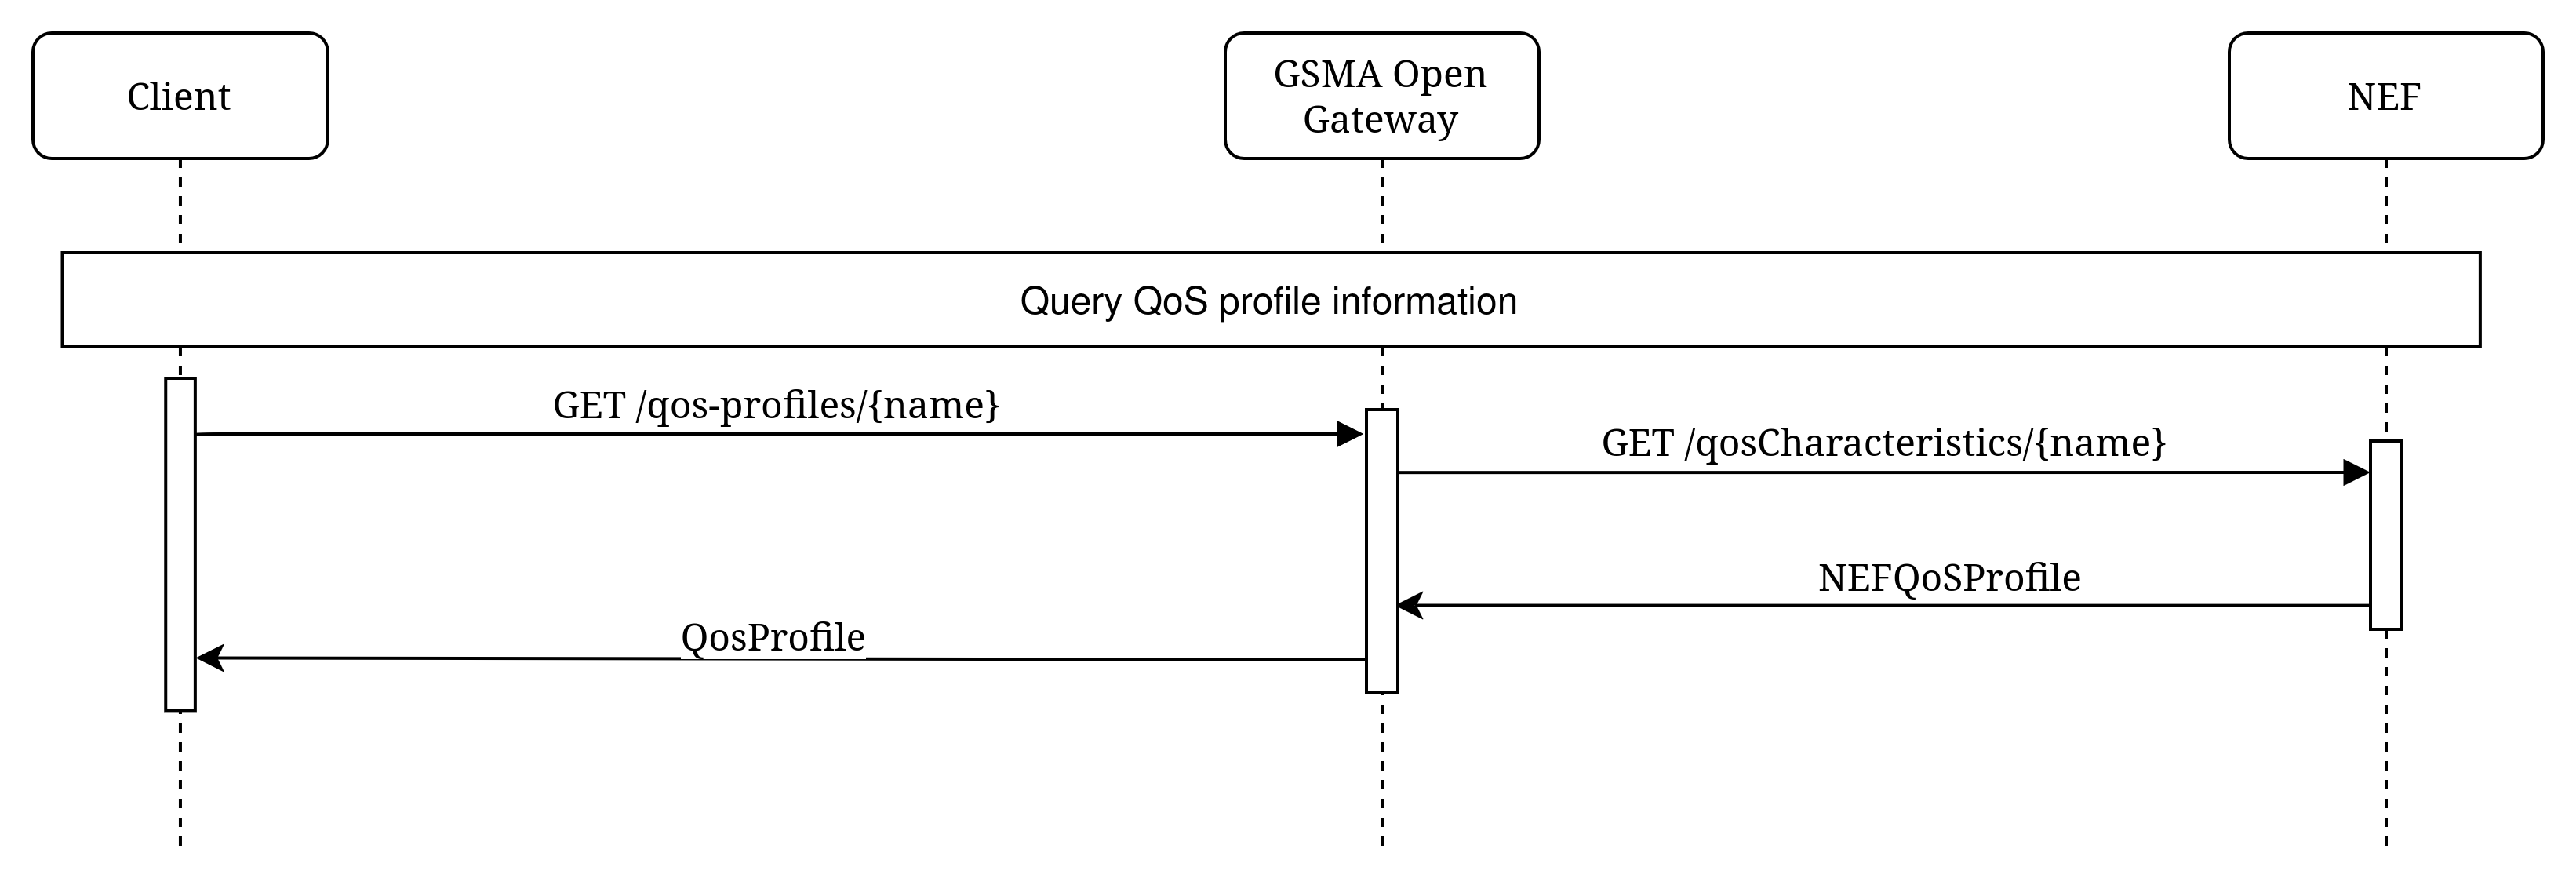
\includegraphics[width=10cm]{figs/QoS_profiles_sequence_diagram.png}
	}
	\caption{Quality of Service Profiles Sequence Diagram}
\end{figure}
